\documentclass[a4paper,11pt]{article}

%%%%%%%%%%%%%%%%%%%%%%%%%%%%%%%%%%%%%%%%%%%%%%%%%%%%%%%%%%%%%%%%%%%%%%%%
% Paquetes utilizados
%%%%%%%%%%%%%%%%%%%%%%%%%%%%%%%%%%%%%%%%%%%%%%%%%%%%%%%%%%%%%%%%%%%%%%%%

% Graficos complejos
\usepackage{graphicx}
\usepackage{caption}
\usepackage{subcaption}
\usepackage{placeins}

% Soporte para el lenguaje español
\usepackage{textcomp}
\usepackage[utf8]{inputenc}
\usepackage[T1]{fontenc}
\DeclareUnicodeCharacter{B0}{\textdegree}
\usepackage[spanish]{babel}

% Matematicos
\usepackage{amssymb,amsmath}

% Soporte para arrays y tabs y formatos de columna
\usepackage{array}

% Soporte para subrayado
\usepackage{ulem}

% Soporte para enumerados
\usepackage{enumerate}

% PDFs embebidos para el apendice
\usepackage{pdfpages}

% Soporte para warnings
\usepackage{fixltx2e}

% Soporte para headers y footers
\usepackage{fancyhdr}
\renewcommand{\headrulewidth}{0pt}
\renewcommand{\footrulewidth}{0pt}
\usepackage{color}

\definecolor{color01}{rgb}{0.40,0.40,0.40}

\newcommand{\tab}{\hspace{5mm}}

% Formato de parrafo
\setlength{\parskip}{1ex plus 0.5ex minus 0.2ex}

%%%%%%%%%%%%%%%%%%%%%%%%%%%%%%%%%%%%%%%%%%%%%%%%%%%%%%%%%%%%%%%%%%%%%%%%
% Titulo
%%%%%%%%%%%%%%%%%%%%%%%%%%%%%%%%%%%%%%%%%%%%%%%%%%%%%%%%%%%%%%%%%%%%%%%%

% Titulo principal del documento.
\title{\textbf{Trabajo Práctico 1: Colas}}

% Informacion sobre los autores.
\author{\\
  Cesar Buffevant, \textit{P. ??.???}                              \\
  \texttt{buffevant@gmail.com}                                     \\ [2.5ex]
  Juan Pecora, \textit{P. ??.???}                                  \\
  \texttt{jlopezpecora@gmail.com}                                  \\ [2.5ex]
  Flavio Olivieri, \textit{P. ??.???}                              \\
  \texttt{flavio.olivieri@gmail.com}                               \\ [2.5ex]
  Sergio Matias Piano, \textit{P. 85.191}                          \\
  \texttt{smpiano@gmail.com}                                       \\ [2.5ex]
  Florencia Tristant, \textit{P. ??.???}                           \\
  \texttt{flotristant@gmail.com}                                   \\ [2.5ex]
  \normalsize{1er. Cuatrimestre de 2015}                           \\
  \normalsize{71.15 Modelos y Optimización 2}                      \\
  \normalsize{Facultad de Ingeniería, Universidad de Buenos Aires} \\
}
\date{}

%%%%%%%%%%%%%%%%%%%%%%%%%%%%%%%%%%%%%%%%%%%%%%%%%%%%%%%%%%%%%%%%%%%%%%%%
% Documento
%%%%%%%%%%%%%%%%%%%%%%%%%%%%%%%%%%%%%%%%%%%%%%%%%%%%%%%%%%%%%%%%%%%%%%%%
\begin{document}
\thispagestyle{empty}
\maketitle

\clearpage

% ----------------------------------------------------------------------
% Tabla de contenidos
% ----------------------------------------------------------------------
\tableofcontents
\clearpage

\part{Resolución de ejercicios}
\section*{\textbf{Ejercicio 1}}

\baselineskip=13pt
En una sastrería hay una sección de arreglo y reforma de la ropa vendida a sus
clientes, que es atendida por un sastre. El número de clientes que requieren
arreglos arriban a dicha sección con una distribución de Poisson con una media
de 24 clientes por hora. Debido a que el servicio es gratuito, todos los
clientes están dispuestos a esperar el tiempo que sea necesario para poder
utilizarlo. El tiempo de atención es en promedio de 2 minutos por cliente,
siendo exponencial la distribución de los tiempos de servicio. Calcular:

\leftskip=36pt
\parindent=-18pt
\begin{enumerate}[a)]
  \item ¿Cual es en promedio, el número de clientes en la sección?

  \item ¿Cuánto tiempo permanece, en promedio, un cliente en la sección?

  \item ¿Cual es la probabilidad de que el sastre esté desocupado?

  \item ¿Cual es en promedio, el número de clientes que están esperando recibir
    el servicio?
\end{enumerate}

\vspace{13pt}
\leftskip=0pt
\parindent=0pt
\subsection*{\textbf{Resolución}}

Como sistema se entiende toda la sección de arreglo y
reforma.

\vspace{5pt}
\subsubsection*{Hipotesis:}

Se verifican las hipótesis de un P/P/1. El enunciado dice explícitamente que
todos los clientes están dispuestos a esperar el tiempo que sea necesario, lo
cual se puede interpretar como una cola con capacidad infinita.

\begin{enumerate}[1.]
  \item Tipo de proceso de arribo de clientes responde a distribución Poisson.
  \item Tipo de proceso de servicio a los clientes en el sistema responde a
    distribución Poisson.
  \item Hay un único canal de atención.
  \item El sistema tiene capacidad infinita.
  \item La disciplina de atención es FIFO.
  \item La población es infinita.
  \item Se forma una única cola frente al canal.
  \item El sistema se encuentra en régimen estacionario.
  \item La población no presenta fenómeno de impaciencia.
\end{enumerate}

\vspace{13pt}
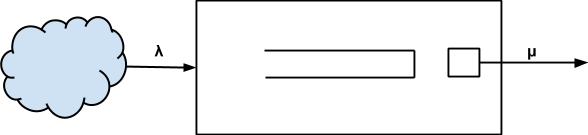
\includegraphics[width=341pt, height=101pt, keepaspectratio=true]{TP1-Colas-fig001.png}

\vspace{27pt}
Parámetros del modelo:

$\lambda = 24 [clientes/hora]$

$T_s = 2 [minutos/cliente] \times \frac{1[hora]}{60[minutos]} = 0.033
[horas/cliente]$ → $\mu = 30 [clientes/hora]$

\begin{enumerate}[a)]
  \vspace{13pt}
  \item El número de clientes en la sección, es decir el número de clientes en
    el sistema, es L.

  $L = \frac{\lambda}{\mu - \lambda} = \frac{24}{30 - 24} = 4 [clientes/hora]$

  \vspace{13pt}
  \item El tiempo que permanece un cliente en la sección, es decir, en el
    sistema es W:

  $W = \frac{1}{\mu-\lambda} = \frac{1}{30-24} = 0,1667[horas] \times \frac{60[minutos]}{1[hora]} = 10[minutos]$

  \vspace{13pt}
  \item La probabilidad de que el sastre esté desocupado es la probabilidad de
    que en la sección no haya nadie, es decir P(0)

  $P(0) = 1-\rho = 1-\frac{24}{30} = 0,2$

  \vspace{13pt}
  \item El número de clientes esperando recibir el servicio son los clientes
    que están en la cola, es decir $L_c$.

  $L_c = \frac{\rho^2}{1-\rho} = \frac{0,64}{1-0,8} = 3,2$

\end{enumerate}
\vspace{35pt}
\section*{\textbf{Ejercicio 2}}

Un establecimiento de reparaciones, atendido por un solo operario, recibe un
promedio de cuatro clientes por hora, los cuales traen pequeños aparatos para
reparar.  El mecanico los inspecciona para encontrar defectos y muy a menudo
puede arreglarlos de inmediato, o de otro modo emitir un diagnostico. En
promedio, todo le toma 6 minutos por aparato. Los arribos tienen una
distribución de de Poisson y el tiempo de servicio tiene una distribución
exponencial. Calcular:

\leftskip=36pt
\parindent=-18pt
\begin{enumerate}[a)]
  \item La probabilidad de que el taller esté vacío.
  \item La probabilidad de que tres clientes estén en el taller.
  \item La probabilidad de encontrar por lo menos un cliente en el taller.
  \item El número promedio de clientes en el taller.
  \item El tiempo promedio que un cliente debe permanecer en el taller.
  \item El número promedio de clientes que esperan ser atendidos.
  \item El tiempo promedio que un cliente debe esperar para ser atendido.
\end{enumerate}

\vspace{13pt}
\leftskip=0pt
\parindent=0pt
\subsection*{\textbf{Resolución}}

Consideramos el sistema como el taller, con el operario incluido. El enunciado
no dice nada con respecto a la capacidad de la cola, por lo que entendemos que
hay suficiente lugar como para albergar a toda la gente que arribe. Responde al
modelo P/P/1

\vspace{5pt}
\subsubsection*{Hipotesis:}

\begin{enumerate}[1.]
  \item Tipo de proceso de arribo de clientes responde a distribución Poisson.
  \item Tipo de proceso de servicio a los clientes en el sistema responde a
    distribución Poisson.
  \item Hay un único canal de atención.
  \item El sistema tiene capacidad infinita.
  \item La disciplina de atención es FIFO.
  \item La población es infinita.
  \item Se forma una única cola frente al canal.
  \item El sistema se encuentra en régimen estacionario.
  \item La población no presenta fenómeno de impaciencia.
\end{enumerate}

\vspace{13pt}
Parámetros del modelo:

$\lambda = 4 [clientes/hora]$

$T_s = 6 [minutos/cliente] \times \frac{1[hora]}{60[minutos]} = 0,1
[horas/cliente]$ → $\mu = 10 [clientes/hora]$.

\begin{enumerate}[a)]
  \vspace{13pt}
  \item La probabilidad de que el taller esté vacío es la probabilidad de que
    no haya ningún cliente en el sistema, es decir $P(0)$.

  $P(0) = 1-\rho = 1-\frac{4}{10} = 0,6$

  \vspace{13pt}
  \item La probabilidad de que tres cliente estén en el sistema es

  $P(3) = \rho^3 (1-\rho) = 0,4^3 \times 0,6 = 0,0384$

  \item La probabilidad de encontrar por lo menos a un cliente es

  $P(n > 0) = 1 - P(0) = 1 - 0.6 = 0.4.$

  \vspace{13pt}
  \item El número promedio de clientes en el taller es el número promedio de
    clientes en el sistema, es decir L.

  $L = \frac{\rho}{1-\rho} = \frac{0,4}{1-0,4} = 0,667$

  \vspace{13pt}
  \item El tiempo promedio que un cliente debe permanecer en el taller es el
    tiempo que un cliente debe permanecer en el sistema, es decir W.

  $W = \frac{1}{\mu-\lambda} = \frac{1}{10-4} = 0,1667[horas/cliente] \times
  \frac{60[minutos]}{1[hora]} = 10[minutos/cliente] $

  \vspace{13pt}
  \item El número de clientes que esperan ser atendidos son los clientes
    esperando en la cola, es decir $L_c$.

  $L_c = \frac{\rho^2}{1-\rho} = \frac{0,16}{1-0,4} = 0,2667$

  \vspace{13pt}
  \item El tiempo promedio que un cliente tiene que esperar para ser atendido
    es el tiempo que pasa en la cola, es decir $W_c$.

    $W_c = \frac{\lambda}{\mu(\mu-\lambda)} = \frac{4}{10\times(10-4)} =
    0,0667[horas/cliente] \times \frac{60[minutos]}{1[hora]} =
    4[minutos/cliente]$

\end{enumerate}

\vspace{35pt}
\section*{\textbf{Ejercicio 3}}

Un banco está desarrollando la prestación de un nuevo servicio, para lo cual ha
habilitado una ventanilla. Como el desarrollo del mismo está basado en una
campaña publicitaria que hace mención al mínimo tiempo de espera que se
requiere, el gerente de la sucursal ha decidido encarar el estudio científico
del problema a fin de no exponerse a un fracaso. Hasta ahora se cuenta con los
siguientes datos:

\leftskip=36pt
\parindent=-18pt
\begin{itemize}
  \item Lapso medio entre arribo de usuarios: 8 minutos (distribución
    exponencial)
  \item Tiempo medio de atención en ventanilla: 2 minutos (distribución
    exponencial).
\end{itemize}

\leftskip=0pt
\parindent=0pt
Determinar:

\leftskip=36pt
\parindent=-18pt
\begin{enumerate}[a)]
  \item La probabilidad de esperar.
  \item La longitud promedio de la cola.
  \item La velocidad promedio de arribos que haría que el tiempo de espera en
    la cola supere los 4 minutos.
\end{enumerate}

\vspace{13pt}
\leftskip=0pt
\parindent=0pt
\subsection*{\textbf{Resolución}}

Consideramos el sistema como la ventanilla más la cola. El enunciado no dice
nada con respecto a la capacidad de la cola, por lo que entendemos que hay
suficiente lugar como para albergar a toda la gente que arribe.

\vspace{5pt}
\subsubsection*{Hipotesis:}

Se verifican las hipótesis de un P/P/1.

\begin{enumerate}[1.]
  \item Tipo de proceso de arribo de clientes responde a distribución Poisson.
  \item Tipo de proceso de servicio a los clientes en el sistema responde a
    distribución Poisson.
  \item Hay un único canal de atención.
  \item El sistema tiene capacidad infinita.
  \item La disciplina de atención es FIFO.
  \item La población es infinita.
  \item Se forma una única cola frente al canal.
  \item El sistema se encuentra en régimen estacionario.
  \item La población no presenta fenómeno de impaciencia.
\end{enumerate}

\vspace{13pt}
Parámetros del modelo:

$T = 8 [minutos/cliente]$ →  $\lambda = 0,125 [clientes/minuto]$.

$Ts = 2 [minutos/cliente]$ → $\mu = 0,5 [clientes/minuto]$.

\begin{enumerate}[a)]
  \vspace{13pt}
  \item La probabilidad de esperar es la probabilidad de que en el sistema haya
    algún cliente, es decir $P(n>0) = 1 - P(0)$.

  $P(n>0) = 1 - P(0) = 1-1+\rho = \frac{\lambda}{\mu} = \frac{0,125}{0,5} =
  0,25$

  \vspace{13pt}
  \item La longitud promedio de la cola es la cantidad de clientes en promedio
    esperando para ser atendidos, es decir $L_c$.

  $L_c = \frac{\lambda^2}{\mu(\mu-\lambda)} = \frac{0,125^2}{0,5 \times
  (0,5-0,125)} = 0,0833$

  \vspace{13pt}
  \item El tiempo de espera en la cola es $W_c$, es decir:

  $W_c = \frac{\lambda}{\mu(\mu-\lambda)} < 4 \implies \lambda < 4
  \mu(\mu-\lambda) \implies \lambda < 4 \mu^2-4\mu\lambda \implies \lambda +
  4\mu\lambda < 4 \mu^2 \implies \lambda(1 + 4\mu) < 4\mu^2 \implies \lambda <
  \frac{4\mu^2}{1+4\mu}$

  $\lambda < \frac{4\mu^2}{1+4\mu} = \frac{4\times0,5^2}{1+4\times0,5} =
  0,333[clientes/minuto]$
\end{enumerate}

\vspace{35pt}
\section*{\textbf{Ejercicio 4}}

Teniendo en cuenta el ejercicio 2, considerar todas las suposiciones
anteriores, excepto que si hay tres clientes en el taller, cualquier otro
cliente que llegue se retirará.

Determinar entonces:

\leftskip=36pt
\parindent=-18pt
\begin{enumerate}[a)]
  \item La probabilidad de que el taller esté vacío.
  \item La probabilidad de que tres clientes estén en el taller.
  \item La probabilidad de encontrar por lo menos un cliente en el taller.
  \item El número promedio de clientes en el taller.
  \item El tiempo promedio que un cliente debe permanecer en el taller.
  \item El número promedio de clientes que esperan ser atendidos.
  \item El tiempo promedio que un cliente debe esperar para ser atendido.
  \item La cantidad promedio de clientes que se retiran sin ser atendidos.
\end{enumerate}

\vspace{13pt}
\leftskip=0pt
\parindent=0pt
\subsection*{\textbf{Resolución}}

\vspace{5pt}
\leftskip=0pt
\parindent=0pt
\subsubsection*{Hipótesis:}

\leftskip=36pt
\parindent=-18pt
\begin{itemize}
  \item El proceso de llegada de los clientes responde a un proceso Poisson.
  \item El proceso de atención de los clientes responde a un proceso Poisson.
  \item La población es infinita
  \item Se forma una única cola frente al canal de atención.
  \item Existe un único canal de atención.
  \item La capacidad del sistema es infinita
  \item La atención de los clientes de la cola es FIFO
  \item El sistema se encuentra en condiciones estables.
  \item \textit{La población presenta el fenómeno de impaciencia.}
\end{itemize}

\vspace{21pt}
\leftskip=0pt
\parindent=0pt
\textit{Sistema}

El sistema se modela como un sistema PP1 con impaciencia:

\vspace{13pt}
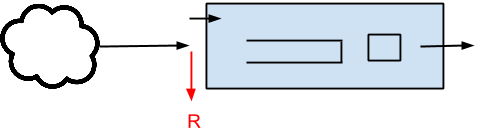
\includegraphics[width=359pt, height=99pt, keepaspectratio=true]{TP1-Colas-fig002.png}

$\lambda = 7,5[clientes/hora]$

$\mu = 30[clientes/hora]$


\vspace{27pt}
\begin{tabular}{|>{\centering}p{33pt}|>{\centering}p{31pt}|>{\centering}p{31pt}|>{\centering}p{31pt}|>{\centering}p{31pt}|>{\centering}p{31pt}|>{\centering}p{31pt}|>{\centering}p{31pt}|}
\hline
$n$ & $P(n)$ & $\lambda$ & $\mu$ & $L$ & $Lc$ & $H$ & $R$\tabularnewline
\hline
0 & $P(0)$ & $\lambda$ & 0 & 0 & 0 & 0 & 0\tabularnewline
\hline
1 & $P(1)$ & $\lambda$ & $\mu$ & 1 & 0 & 1 & 0\tabularnewline
\hline
2 & $P(2)$ & $\lambda$ & $\mu$ & 2 & 1 & 1 & 0\tabularnewline
\hline
3 & $P(3)$ & 0 & $\mu$ & 3 & 2 & 1 & $\lambda$\tabularnewline
\hline
4 & $P(4)$ & 0 & $\mu$ & 3 & 2 & 1 & $\lambda$\tabularnewline
\hline
5 & 0 & 0 & $\mu$ & 3 & 2 & 1 & $\lambda$\tabularnewline
\hline
.. & .. & ... & ... & ... & ... & ... & ...\tabularnewline
\hline
\end{tabular}

\vspace{13pt}
\leftskip=36pt
\parindent=-18pt
\begin{enumerate}[a)]
  \item 
    $P(1) = \frac{\lambda P(0)}{\mu} = \rho P(0)$ 

    $P(2) = \frac{\lambda P(1)}{\mu} = \rho^2P(0)$ 

    $P(3) = \frac{\lambda P(2)}{\mu} = \rho^3P(0)$ 

    $\rho = \frac{\lambda}{\mu} = \frac{7,5[clientes/hora]}{30[clientes/hora]}
    = 0,25$

    $P(0) + P(1) + P(2) +P(3) = 1 \implies P(0) =
    \frac{1}{1+\rho+\rho^2+\rho^3} = 0,75$
   

  \vspace{13pt}
  \item
    $P(3) = \rho^3P(0) = 0,012$ 

  \vspace{13pt}
  \item
    $1-P(0) = 1-0,75 = 0,25$ 

  \vspace{13pt}
  \item
    $L = 1 \times P(1) + 2 \times P(2) + 3 \times P(3) = 0,75
    \times(\rho+2\rho^2+3\rho^3) = 0,32$ 

  \vspace{13pt}
  \item
    $H = P(1) + P(2) + P(3) = 1 - P(0) = 0,25$ 

    $L_c = L - H = 0,52 - 0,25 = 0,27$ 

    $\lambda = \lambda(P(0) + P(1) + P(2)) = \lambda(1-P(3)) = \lambda(1-0,012)
    = 7,41 [clientes/hora]$ 

    $W = W_c + T_s = \frac{L_c}{\lambda} + \frac{1}{\mu} =
    \frac{0,27}{7,41[clientes/hora]} + \frac{1}{30[clientes/hora]} =
    0,069[horas/cliente] \times \frac{60[minutos]}{1[hora]} =
    4,18[minutos/cliente]$

  \item
    $L_c = 0,27$

  \item
    $\overline{\lambda} = \lambda(P(0) + P(1) + P(2)) = \lambda(1-P(3)) =
    \lambda(1-0,012) = 7,41[clientes/hora]$

    $W_c = \frac{L_c}{\lambda} = \frac{0,27}{7,41[clientes/hora]} =
    0,036[horas/cliente] \times \frac{60[minutos]}{1[hora]} =
    2,18[minutos/cliente]$

  \item
    $R = \lambda P(3) = 0,09[clientes/hora]$
\end{enumerate}

%\vspace{21pt}
%\subsubsection*{{\color{color01} \textbf{Ejercicio 5}}}
%
%\leftskip=0pt
%\parindent=0pt
%Una empresa tiene cuatro máquinas cortadoras de césped. Las mismas se rompen 
%o necesitan
%
%mantenimiento cada 15 días (distribución exponencial). Para su atención y mantenimiento 
%tiene
%
%un empleado que en promedio tarda 7 días con cada máquina. En promedio, por cada 
%día de
%
%trabajo, las máquinas reportan un ingreso de \$50. Se desea saber:
%
%a) El número promedio de máquinas funcionando.
%
%b) El porcentaje de tiempo que el empleado se encuentra inactivo.
%
%c) Cuánto tiempo, en promedio, estarÁ en funcionamiento una mÁquina.
%
%d) Existe la posibilidad de contratar una persona más, que cobra 700\$ por mes 
%y que tarda lo
%
%mismo que el empleado. Considerando 1 mes = 24 días, ¿conviene contratar al nuevo
%
%empleado?\label{h.xt2hsxra9i77}
%
%\vspace{21pt}
%{\color{color01} \emph{Hipótesis}}
%
%\leftskip=36pt
%\parindent=-18pt
%●\tab El proceso de llegada de los clientes responde a un proceso Poisson.
%
%●\tab El proceso de atención de los clientes responde a un proceso Poisson.
%
%●\tab La población es infinita
%
%●\tab Se forma una única cola frente al canal de atención.
%
%●\tab Existe un único canal de atención.
%
%●\tab La capacidad del sistema es \emph{finita}
%
%●\tab La atención de los clientes de la cola es FIFO
%
%●\tab El sistema se encuentra en condiciones estables.
%
%●\tab La población no presenta el fenómeno de impaciencia.\label{h.btwxbvuxsggy}
%
%\vspace{21pt}
%\leftskip=0pt
%\parindent=0pt
%{\color{color01} \emph{Modelo}}
%
%Este problema es un modelo de población finita:  PP1(N') con N'=4
%
%%%\begin{figure}[htbp]
%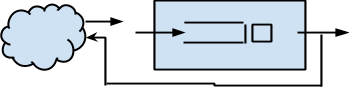
\includegraphics[width=262pt, height=67pt, keepaspectratio=true]{TP1-Colas-fig048.png}
%%%\caption{This should be the caption for \texttt{TP1-Colas-fig048.png}.}
%%%\end{figure}
%
%\vspace{13pt}
%%%\begin{figure}[htbp]
%\includegraphics[width=91pt, height=14pt, keepaspectratio=true]{TP1-Colas-fig049.png}
%%%\caption{This should be the caption for \texttt{TP1-Colas-fig049.png}.}
%%%\end{figure}
%
%\vspace{27pt}
%\begin{tabular}{|>{\raggedright}p{28pt}|>{\raggedright}p{26pt}|>{\raggedright}p{26pt}|>{\raggedright}p{26pt}|>{\raggedright}p{26pt}|>{\raggedright}p{26pt}|>{\raggedright}p{26pt}|>{\raggedright}p{26pt}|>{\raggedright}p{26pt}|}
%\hline
%n & P(n)
%\includegraphics[width=8pt, height=11pt, keepaspectratio=true]{TP1-Colas-fig050.png}
% & 
%\includegraphics[width=8pt, height=11pt, keepaspectratio=true]{TP1-Colas-fig051.png}
% &  & L & Lc & J & N' & H\tabularnewline
%\hline
%0 & P(0)
%\includegraphics[width=24pt, height=14pt, keepaspectratio=true]{TP1-Colas-fig052.png}
% &  & 0 & 0 & 0 & 4 & 4 & 0\tabularnewline
%\hline
%1 & P(1)
%\includegraphics[width=24pt, height=14pt, keepaspectratio=true]{TP1-Colas-fig053.png}
% & 
%\includegraphics[width=8pt, height=11pt, keepaspectratio=true]{TP1-Colas-fig054.png}
% &  & 1 & 0 & 3 & 4 & 1\tabularnewline
%\hline
%2 & P(2)
%\includegraphics[width=24pt, height=14pt, keepaspectratio=true]{TP1-Colas-fig055.png}
% & 
%\includegraphics[width=8pt, height=11pt, keepaspectratio=true]{TP1-Colas-fig056.png}
% &  & 2 & 1 & 2 & 4 & 1\tabularnewline
%\hline
%3 & P(3)
%\includegraphics[width=17pt, height=14pt, keepaspectratio=true]{TP1-Colas-fig057.png}
% & 
%\includegraphics[width=8pt, height=11pt, keepaspectratio=true]{TP1-Colas-fig058.png}
% &  & 3 & 2 & 1 & 4 & 1\tabularnewline
%\hline
%4 & P(4) & 0
%\includegraphics[width=8pt, height=11pt, keepaspectratio=true]{TP1-Colas-fig059.png}
% &  & 4 & 3 & 0 & 4 & 1\tabularnewline
%\hline
%.. & 0 & .. & .. & .. & .. & .. & .. & ..\tabularnewline
%\hline
%\end{tabular}
%
%\vspace{13pt}
%\leftskip=36pt
%\parindent=-18pt
%a.\tab 
%\includegraphics[width=199pt, height=14pt, keepaspectratio=true]{TP1-Colas-fig060.png}
%
%%%\begin{figure}[htbp]
%\includegraphics[width=158pt, height=29pt, keepaspectratio=true]{TP1-Colas-fig061.png}
%%%\caption{This should be the caption for \texttt{TP1-Colas-fig061.png}.}
%%%\end{figure}
%
%\vspace{13pt}
%%%\begin{figure}[htbp]
%\includegraphics[width=167pt, height=29pt, keepaspectratio=true]{TP1-Colas-fig062.png}
%%%\caption{This should be the caption for \texttt{TP1-Colas-fig062.png}.}
%%%\end{figure}
%
%\vspace{13pt}
%%%\begin{figure}[htbp]
%\includegraphics[width=170pt, height=29pt, keepaspectratio=true]{TP1-Colas-fig063.png}
%%%\caption{This should be the caption for \texttt{TP1-Colas-fig063.png}.}
%%%\end{figure}
%
%\vspace{13pt}
%%%\begin{figure}[htbp]
%\includegraphics[width=164pt, height=29pt, keepaspectratio=true]{TP1-Colas-fig064.png}
%%%\caption{This should be the caption for \texttt{TP1-Colas-fig064.png}.}
%%%\end{figure}
%
%\vspace{13pt}
%%%\begin{figure}[htbp]
%\includegraphics[width=155pt, height=32pt, keepaspectratio=true]{TP1-Colas-fig065.png}
%%%\caption{This should be the caption for \texttt{TP1-Colas-fig065.png}.}
%%%\end{figure}
%
%\vspace{13pt}
%%%\begin{figure}[htbp]
%\includegraphics[width=461pt, height=29pt, keepaspectratio=true]{TP1-Colas-fig066.png}
%%%\caption{This should be the caption for \texttt{TP1-Colas-fig066.png}.}
%%%\end{figure}
%
%\vspace{13pt}
%%%\begin{figure}[htbp]
%\includegraphics[width=59pt, height=11pt, keepaspectratio=true]{TP1-Colas-fig067.png}
%%%\caption{This should be the caption for \texttt{TP1-Colas-fig067.png}.}
%%%\end{figure}
%
%\vspace{13pt}
%b.\tab 
%\includegraphics[width=77pt, height=14pt, keepaspectratio=true]{TP1-Colas-fig068.png}
%
%c.\tab 
%\includegraphics[width=518pt, height=14pt, keepaspectratio=true]{TP1-Colas-fig069.png}
%
%\includegraphics[width=156pt, height=19pt, keepaspectratio=true]{TP1-Colas-fig070.png}
%
%d.\tab Para saber si conviene contratar un nuevo empleado a \$700 por mes, se plantea 
%un nuevo sistema con 2 canales: PPMN:\label{h.we0rz647mwgh}
%
%\vspace{21pt}
%\leftskip=0pt
%\parindent=0pt
%{\color{color01} \emph{Hipótesis}}
%
%\leftskip=36pt
%\parindent=-18pt
%●\tab El proceso de llegada de los clientes responde a un proceso Poisson.
%
%●\tab El proceso de atención de los clientes responde a un proceso Poisson.
%
%●\tab La población es infinita
%
%●\tab Se forma una única cola frente al canal de atención.
%
%●\tab \emph{Hay dos canales de atención}
%
%●\tab La capacidad del sistema es \emph{finita}
%
%●\tab La atención de los clientes de la cola es FIFO
%
%●\tab El sistema se encuentra en condiciones estables.
%
%●\tab La población no presenta el fenómeno de impaciencia.\label{h.oy764fhdy6s9}
%
%\vspace{21pt}
%\leftskip=0pt
%\parindent=0pt
%{\color{color01} \emph{Modelo}}
%
%Este problema es un modelo de población finita:  PP1(N') con N'=4
%
%%%\begin{figure}[htbp]
%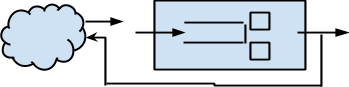
\includegraphics[width=262pt, height=67pt, keepaspectratio=true]{TP1-Colas-fig071.png}
%%%\caption{This should be the caption for \texttt{TP1-Colas-fig071.png}.}
%%%\end{figure}
%
%\vspace{13pt}
%%%\begin{figure}[htbp]
%\includegraphics[width=91pt, height=14pt, keepaspectratio=true]{TP1-Colas-fig072.png}
%%%\caption{This should be the caption for \texttt{TP1-Colas-fig072.png}.}
%%%\end{figure}
%
%\vspace{55pt}
%\begin{tabular}{|>{\raggedright}p{28pt}|>{\raggedright}p{26pt}|>{\raggedright}p{26pt}|>{\raggedright}p{26pt}|>{\raggedright}p{26pt}|>{\raggedright}p{26pt}|>{\raggedright}p{26pt}|>{\raggedright}p{26pt}|>{\raggedright}p{26pt}|}
%\hline
%n & P(n)
%\includegraphics[width=8pt, height=11pt, keepaspectratio=true]{TP1-Colas-fig073.png}
% & 
%\includegraphics[width=8pt, height=11pt, keepaspectratio=true]{TP1-Colas-fig074.png}
% &  & L & Lc & J & N' & H\tabularnewline
%\hline
%0 & P(0)
%\includegraphics[width=24pt, height=14pt, keepaspectratio=true]{TP1-Colas-fig075.png}
% & 8
%\includegraphics[width=24pt, height=14pt, keepaspectratio=true]{TP1-Colas-fig076.wmf}
% & 0 & 0 & 0 & 4 & 4 & 0\tabularnewline
%\hline
%1 & P(1)
%\includegraphics[width=24pt, height=14pt, keepaspectratio=true]{TP1-Colas-fig077.png}
% & 8
%\includegraphics[width=24pt, height=14pt, keepaspectratio=true]{TP1-Colas-fig078.wmf}
%
%\includegraphics[width=8pt, height=11pt, keepaspectratio=true]{TP1-Colas-fig079.png}
% &  & 1 & 0 & 3 & 4 & 1\tabularnewline
%\hline
%2 & P(2)
%\includegraphics[width=24pt, height=14pt, keepaspectratio=true]{TP1-Colas-fig080.png}
% & 8
%\includegraphics[width=24pt, height=14pt, keepaspectratio=true]{TP1-Colas-fig081.wmf}
%
%\includegraphics[width=15pt, height=14pt, keepaspectratio=true]{TP1-Colas-fig082.png}
% &  & 2 & 1 & 2 & 4 & 1\tabularnewline
%\hline
%3 & P(3)
%\includegraphics[width=17pt, height=14pt, keepaspectratio=true]{TP1-Colas-fig083.png}
% & 8
%\includegraphics[width=17pt, height=14pt, keepaspectratio=true]{TP1-Colas-fig084.wmf}
%
%\includegraphics[width=15pt, height=14pt, keepaspectratio=true]{TP1-Colas-fig085.png}
% &  & 3 & 2 & 1 & 4 & 1\tabularnewline
%\hline
%4 & P(4) & 0
%\includegraphics[width=15pt, height=14pt, keepaspectratio=true]{TP1-Colas-fig086.png}
% &  & 4 & 3 & 0 & 4 & 1\tabularnewline
%\hline
%.. & 0 & .. & .. & .. & .. & .. & .. & ..\tabularnewline
%\hline
%\end{tabular}
%
%\vspace{27pt}
%%%\begin{figure}[htbp]
%\includegraphics[width=199pt, height=14pt, keepaspectratio=true]{TP1-Colas-fig087.png}
%%%\caption{This should be the caption for \texttt{TP1-Colas-fig087.png}.}
%%%\end{figure}
%
%\vspace{13pt}
%%%\begin{figure}[htbp]
%\includegraphics[width=158pt, height=29pt, keepaspectratio=true]{TP1-Colas-fig088.png}
%%%\caption{This should be the caption for \texttt{TP1-Colas-fig088.png}.}
%%%\end{figure}
%
%\vspace{13pt}
%%%\begin{figure}[htbp]
%\includegraphics[width=161pt, height=31pt, keepaspectratio=true]{TP1-Colas-fig089.png}
%%%\caption{This should be the caption for \texttt{TP1-Colas-fig089.png}.}
%%%\end{figure}
%
%\vspace{13pt}
%%%\begin{figure}[htbp]
%\includegraphics[width=162pt, height=31pt, keepaspectratio=true]{TP1-Colas-fig090.png}
%%%\caption{This should be the caption for \texttt{TP1-Colas-fig090.png}.}
%%%\end{figure}
%
%\vspace{13pt}
%%%\begin{figure}[htbp]
%\includegraphics[width=156pt, height=31pt, keepaspectratio=true]{TP1-Colas-fig091.png}
%%%\caption{This should be the caption for \texttt{TP1-Colas-fig091.png}.}
%%%\end{figure}
%
%\vspace{13pt}
%%%\begin{figure}[htbp]
%\includegraphics[width=155pt, height=32pt, keepaspectratio=true]{TP1-Colas-fig092.png}
%%%\caption{This should be the caption for \texttt{TP1-Colas-fig092.png}.}
%%%\end{figure}
%
%\vspace{13pt}
%%%\begin{figure}[htbp]
%\includegraphics[width=446pt, height=29pt, keepaspectratio=true]{TP1-Colas-fig093.png}
%%%\caption{This should be the caption for \texttt{TP1-Colas-fig093.png}.}
%%%\end{figure}
%
%\vspace{13pt}
%%%\begin{figure}[htbp]
%\includegraphics[width=60pt, height=14pt, keepaspectratio=true]{TP1-Colas-fig094.png}
%%%\caption{This should be the caption for \texttt{TP1-Colas-fig094.png}.}
%%%\end{figure}
%
%\vspace{27pt}
%%%\begin{figure}[htbp]
%\includegraphics[width=140pt, height=14pt, keepaspectratio=true]{TP1-Colas-fig095.png}
%%%\caption{This should be the caption for \texttt{TP1-Colas-fig095.png}.}
%%%\end{figure}
%
%8
%\includegraphics[width=140pt, height=14pt, keepaspectratio=true]{TP1-Colas-fig096.wmf}
%
%Antes:
%
%%%\begin{figure}[htbp]
%\includegraphics[width=458pt, height=15pt, keepaspectratio=true]{TP1-Colas-fig097.png}
%%%\caption{This should be the caption for \texttt{TP1-Colas-fig097.png}.}
%%%\end{figure}
%
%\vspace{13pt}
%Ahora:
%
%%%\begin{figure}[htbp]
%\includegraphics[width=461pt, height=15pt, keepaspectratio=true]{TP1-Colas-fig098.png}
%%%\caption{This should be the caption for \texttt{TP1-Colas-fig098.png}.}
%%%\end{figure}
%
%\vspace{27pt}
%%%\begin{figure}[htbp]
%\includegraphics[width=344pt, height=14pt, keepaspectratio=true]{TP1-Colas-fig099.png}
%%%\caption{This should be the caption for \texttt{TP1-Colas-fig099.png}.}
%%%\end{figure}
%
%8
%\includegraphics[width=344pt, height=14pt, keepaspectratio=true]{TP1-Colas-fig100.wmf}
%
%{\color{color01} \textbf{Ejercicio 6}}
%
%Una peluquería tiene un peluquero que realiza un corte de pelo especial a los 
%clientes. Recientemente se ha contratado un aprendiz para que lo ayude, decidiendo 
%que solo realice el corte cuando llega el segundo cliente a la cola de espera. 
%Tanto el peluquero como el aprendiz demoran en promedio media hora cada uno para 
%atender a cada cliente. Al local llegan en promedio 5 clientes por hora (distribución 
%Poisson). Los clientes son impacientes. Si hay un cliente esperando, solamente 
%el 50\% de los clientes que llegan deciden entrar a la peluquería. Si hay más 
%de un cliente esperando, no entra ningún cliente más ya que no estÁn dispuestos 
%a esperar. Se pide calcular: 
%
%a) La probabilidad de que no haya clientes en la peluquería. 
%
%b) La probabilidad de que haya clientes esperando para recibir el servicio. 
%
%c) El porcentaje de ocupación del peluquero y del aprendiz. 
%
%d) La cantidad promedio de clientes esperando para recibir el servicio. 
%
%e) La cantidad promedio de clientes que no ingresan a la peluquería. 
%
%f) Si cada corte de pelo cuesta 30\$, calcular el ingreso económico promedio de 
%la peluquería, por hora.
%
%\vspace{13pt}
%{\color{color01} \emph{Modelo}}
%
%\vspace{13pt}
%Este problema es un modelo P/P/2 con impaciencia 
%
%\vspace{13pt}
%%%\begin{figure}[htbp]
%\includegraphics[width=343pt, height=102pt, keepaspectratio=true]{TP1-Colas-fig101.png}
%%%\caption{This should be the caption for \texttt{TP1-Colas-fig101.png}.}
%%%\end{figure}
%
%\label{h.dot8ji50046r}
%
%\vspace{21pt}
%{\color{color01} \emph{Hipótesis}}
%
%\leftskip=36pt
%\parindent=-18pt
%●\tab El proceso de llegada de los clientes responde a un proceso Poisson.
%
%●\tab El proceso de atención de los clientes responde a un proceso Poisson.
%
%●\tab La población es infinita
%
%●\tab Existen 2 canales de atención.
%
%●\tab Se forma una única cola frente a los canales de atención.
%
%●\tab La capacidad del sistema es in\emph{finita}
%
%●\tab La atención de los clientes de la cola es FIFO
%
%●\tab El sistema se encuentra en condiciones estables.
%
%●\tab La población presenta el fenómeno de impaciencia.
%
%\vspace{13pt}
%\leftskip=0pt
%\parindent=0pt
%{\color{color01} \emph{Datos}}
%
%\leftskip=36pt
%\parindent=-18pt
%●\tab 
%\includegraphics[width=109pt, height=15pt, keepaspectratio=true]{TP1-Colas-fig102.png}
%
%●\tab 
%\includegraphics[width=108pt, height=15pt, keepaspectratio=true]{TP1-Colas-fig103.png}
%
%●\tab Probabilidad de ingreso
%
%\leftskip=72pt
%○\tab n = 0 -\texttt{>} PI = 1
%
%○\tab n = 1 -\texttt{>} PI = 1
%
%○\tab n = 2 -\texttt{>} PI = 0.5
%
%○\tab n = 3 -\texttt{>} PI = 0.5
%
%○\tab n = 4 -\texttt{>} PI = 1
%
%\vspace{13pt}
%\leftskip=0pt
%\parindent=0pt
%{\color{color01} \emph{Resolucion}}
%
%\vspace{13pt}
%\begin{tabular}{|>{\raggedright}p{21pt}|>{\raggedright}p{24pt}|>{\raggedright}p{28pt}|>{\raggedright}p{28pt}|>{\raggedright}p{28pt}|>{\raggedright}p{19pt}|>{\raggedright}p{21pt}|>{\raggedright}p{21pt}|>{\raggedright}p{19pt}|>{\raggedright}p{19pt}|}
%\hline
%\centering n & \centering P(n) & \centering $\lambda$ & \centering $\mu$ & \centering L & \centering Lc & \centering H & \centering R & \centering H1 & \centering H2\tabularnewline
%\hline
%\centering 0 & \centering P(0) & \centering $\lambda$ & \centering 0 & \centering 0 & \centering 0 & \centering 0 & \centering 0 & \centering 0 & \centering 0\tabularnewline
%\hline
%\centering 1 & \centering P(1) & \centering $\lambda$ & \centering $\mu$ & \centering 1 & \centering 0 & \centering 1 & \centering 0 & \centering 1 & \centering 0\tabularnewline
%\hline
%\centering 2 & \centering P(2) & \centering 0.5$\lambda$ & \centering $\mu$ & \centering 2 & \centering 1 & \centering 1 & \centering 0.5$\lambda$ & \centering 1 & \centering 0\tabularnewline
%\hline
%\centering 3 & \centering P(3) & \centering 0.5$\lambda$ & \centering 2$\mu$ & \centering 3 & \centering 1 & \centering 2 & \centering 0.5$\lambda$ & \centering 1 & \centering 1\tabularnewline
%\hline
%\centering 4 & \centering P(4) & \centering 0 & \centering 2$\mu$ & \centering 4 & \centering 2 & \centering 2 & \centering $\lambda$ & \centering 1 & \centering 1\tabularnewline
%\hline
%\end{tabular}
%
%\vspace{27pt}
%%%\begin{figure}[htbp]
%\includegraphics[width=264pt, height=31pt, keepaspectratio=true]{TP1-Colas-fig104.png}
%%%\caption{This should be the caption for \texttt{TP1-Colas-fig104.png}.}
%%%\end{figure}
%
%\vspace{27pt}
%%%\begin{figure}[htbp]
%\includegraphics[width=272pt, height=31pt, keepaspectratio=true]{TP1-Colas-fig105.png}
%%%\caption{This should be the caption for \texttt{TP1-Colas-fig105.png}.}
%%%\end{figure}
%
%8
%\includegraphics[width=272pt, height=31pt, keepaspectratio=true]{TP1-Colas-fig106.wmf}
%
%\vspace{27pt}
%%%\begin{figure}[htbp]
%\includegraphics[width=294pt, height=31pt, keepaspectratio=true]{TP1-Colas-fig107.png}
%%%\caption{This should be the caption for \texttt{TP1-Colas-fig107.png}.}
%%%\end{figure}
%
%\vspace{27pt}
%%%\begin{figure}[htbp]
%\includegraphics[width=297pt, height=31pt, keepaspectratio=true]{TP1-Colas-fig108.png}
%%%\caption{This should be the caption for \texttt{TP1-Colas-fig108.png}.}
%%%\end{figure}
%
%8
%\includegraphics[width=297pt, height=31pt, keepaspectratio=true]{TP1-Colas-fig109.wmf}
%
%\vspace{13pt}
%%%\begin{figure}[htbp]
%\includegraphics[width=572pt, height=24pt, keepaspectratio=true]{TP1-Colas-fig110.png}
%%%\caption{This should be the caption for \texttt{TP1-Colas-fig110.png}.}
%%%\end{figure}
%
%8
%\includegraphics[width=572pt, height=24pt, keepaspectratio=true]{TP1-Colas-fig111.wmf}
%
%\vspace{13pt}
%%%\begin{figure}[htbp]
%\includegraphics[width=251pt, height=37pt, keepaspectratio=true]{TP1-Colas-fig112.png}
%%%\caption{This should be the caption for \texttt{TP1-Colas-fig112.png}.}
%%%\end{figure}
%
%\vspace{27pt}
%a) probabilidad de que no haya clientes en la peluquería
%
%P(0) = 0.0621
%
%b) probabilidad de que haya clientes esperando para recibir el servicio
%
%P(2\texttt{<}n\texttt{<}4) = 0,7826
%
%c) porcentaje de ocupación del peluquero y del aprendiz
%
%\parindent=36pt
%%%\begin{figure}[htbp]
%\includegraphics[width=257pt, height=35pt, keepaspectratio=true]{TP1-Colas-fig113.png}
%%%\caption{This should be the caption for \texttt{TP1-Colas-fig113.png}.}
%%%\end{figure}
%
%\vspace{13pt}
%%%\begin{figure}[htbp]
%\includegraphics[width=261pt, height=35pt, keepaspectratio=true]{TP1-Colas-fig114.png}
%%%\caption{This should be the caption for \texttt{TP1-Colas-fig114.png}.}
%%%\end{figure}
%
%\vspace{27pt}
%\parindent=0pt
%d) cantidad promedio de clientes esperando para recibir el servicio
%
%%%\begin{figure}[htbp]
%\includegraphics[width=0pt, height=0pt, keepaspectratio=true]{TP1-Colas-fig115.???}
%%%\caption{This should be the caption for \texttt{TP1-Colas-fig115.???}.}
%%%\end{figure}
%
%\includegraphics[width=227pt, height=35pt, keepaspectratio=true]{TP1-Colas-fig116.wmf}
%
%\vspace{13pt}
%e) cantidad promedio de clientes que no ingresan a la peluquería
%
%%%\begin{figure}[htbp]
%\includegraphics[width=224pt, height=35pt, keepaspectratio=true]{TP1-Colas-fig117.png}
%%%\caption{This should be the caption for \texttt{TP1-Colas-fig117.png}.}
%%%\end{figure}
%
%\vspace{27pt}
%f) Si cada corte de pelo cuesta 30\$, calcular el ingreso económico promedio de 
%la peluquería
%
%%%\begin{figure}[htbp]
%\includegraphics[width=298pt, height=35pt, keepaspectratio=true]{TP1-Colas-fig118.png}
%%%\caption{This should be the caption for \texttt{TP1-Colas-fig118.png}.}
%%%\end{figure}
%
%\label{h.7ydn9uhtojep}
%
%\vspace{49pt}
%\subsubsection*{{\color{color01} \textbf{Ejercicio 7}}}
%
%Dado el siguiente sistema:
%
%%%\begin{figure}[htbp]
%\includegraphics[width=316pt, height=141pt, keepaspectratio=true]{TP1-Colas-fig119.png}
%%%\caption{This should be the caption for \texttt{TP1-Colas-fig119.png}.}
%%%\end{figure}
%
%\vspace{13pt}
%Datos:
%
%- Arribos de clientes al sistema: 10 clientes/minuto
%
%- Atención en cada canal: A: 0,2 minutos/clientes        
%
%B: 1/3 minutos/clientes                   
%
%C: 1/2 minutos/clientes
%
%- Valor de cada servicio: A: 0 \$/cliente     
%
%B: 5000 \$/cliente     
%
%C: 600 \$/cliente
%
%- La población en el sector A es impaciente, según la siguiente ley:
%
%\vspace{13pt}
%\begin{tabular}{|>{\raggedright}p{18pt}|>{\raggedright}p{12pt}|>{\raggedright}p{18pt}|>{\raggedright}p{15pt}|>{\raggedright}p{9pt}|}
%\hline
%n & 0 & 1 & 2 & 3\tabularnewline
%\hline
%P(I) & 1 & 0.2 & 0.8 & 0\tabularnewline
%\hline
%\end{tabular}\label{h.p6o6fkl3x9ar}
%
%\vspace{21pt}
%{\color{color01} \emph{Resolución}}
%
%\parindent=36pt
%Como el sistema admite rechazo para el caso de la terminal C, se puede plantear 
%el problema como 3 subsistemas independientes y plantear que:
%
%\vspace{13pt}
%\parindent=0pt
%%%\begin{figure}[htbp]
%\includegraphics[width=193pt, height=15pt, keepaspectratio=true]{TP1-Colas-fig120.png}
%%%\caption{This should be the caption for \texttt{TP1-Colas-fig120.png}.}
%%%\end{figure}
%
%\vspace{13pt}
%%%\begin{figure}[htbp]
%\includegraphics[width=116pt, height=17pt, keepaspectratio=true]{TP1-Colas-fig121.png}
%%%\caption{This should be the caption for \texttt{TP1-Colas-fig121.png}.}
%%%\end{figure}
%
%\vspace{13pt}
%%%\begin{figure}[htbp]
%\includegraphics[width=118pt, height=17pt, keepaspectratio=true]{TP1-Colas-fig122.png}
%%%\caption{This should be the caption for \texttt{TP1-Colas-fig122.png}.}
%%%\end{figure}
%
%\vspace{13pt}
%%%\begin{figure}[htbp]
%\includegraphics[width=64pt, height=17pt, keepaspectratio=true]{TP1-Colas-fig123.png}
%%%\caption{This should be the caption for \texttt{TP1-Colas-fig123.png}.}
%%%\end{figure}
%
%\vspace{13pt}
%%%\begin{figure}[htbp]
%\includegraphics[width=63pt, height=17pt, keepaspectratio=true]{TP1-Colas-fig124.png}
%%%\caption{This should be the caption for \texttt{TP1-Colas-fig124.png}.}
%%%\end{figure}
%
%\vspace{13pt}
%%%\begin{figure}[htbp]
%\includegraphics[width=213pt, height=17pt, keepaspectratio=true]{TP1-Colas-fig125.png}
%%%\caption{This should be the caption for \texttt{TP1-Colas-fig125.png}.}
%%%\end{figure}
%
%\vspace{13pt}
%%%\begin{figure}[htbp]
%\includegraphics[width=218pt, height=17pt, keepaspectratio=true]{TP1-Colas-fig126.png}
%%%\caption{This should be the caption for \texttt{TP1-Colas-fig126.png}.}
%%%\end{figure}
%
%\vspace{13pt}
%%%\begin{figure}[htbp]
%\includegraphics[width=218pt, height=17pt, keepaspectratio=true]{TP1-Colas-fig127.png}
%%%\caption{This should be the caption for \texttt{TP1-Colas-fig127.png}.}
%%%\end{figure}
%
%\vspace{69pt}
%\emph{Sistema A: }
%
%\parindent=36pt
%El sistema presenta las características de un modelo PP1 con impaciencia\label{h.czc72qkn3rsf}
%
%\vspace{8pt}
%\parindent=0pt
%{\color{color01} \emph{Hipótesis}}
%
%\leftskip=36pt
%\parindent=-18pt
%●\tab El proceso de llegada de los clientes responde a un proceso Poisson.
%
%●\tab El proceso de atención de los clientes responde a un proceso Poisson.
%
%●\tab La población es infinita
%
%●\tab Se forma una única cola frente al canal de atención.
%
%●\tab Existe un único canal de atención.
%
%●\tab La capacidad del sistema es infinita
%
%●\tab La atención de los clientes de la cola es FIFO
%
%●\tab El sistema se encuentra en condiciones estables.
%
%●\tab \emph{La población presenta el fenómeno de impaciencia.}
%
%\vspace{13pt}
%\leftskip=0pt
%\parindent=0pt
%\begin{tabular}{|>{\raggedright}p{34pt}|>{\raggedright}p{33pt}|>{\raggedright}p{33pt}|>{\raggedright}p{33pt}|>{\raggedright}p{33pt}|>{\raggedright}p{33pt}|>{\raggedright}p{26pt}|>{\raggedright}p{27pt}|}
%\hline
%n & P(n)
%\includegraphics[width=8pt, height=11pt, keepaspectratio=true]{TP1-Colas-fig128.png}
% & 
%\includegraphics[width=8pt, height=11pt, keepaspectratio=true]{TP1-Colas-fig129.png}
% &  & L & Lc & H & R\tabularnewline
%\hline
%0 & P(0)
%\includegraphics[width=14pt, height=14pt, keepaspectratio=true]{TP1-Colas-fig130.png}
% & 8
%\includegraphics[width=14pt, height=14pt, keepaspectratio=true]{TP1-Colas-fig131.wmf}
% & 0 & 0 & 0 & 0 & 0\tabularnewline
%\hline
%1 & P(1)
%\includegraphics[width=31pt, height=16pt, keepaspectratio=true]{TP1-Colas-fig132.png}
% & 8
%\includegraphics[width=31pt, height=16pt, keepaspectratio=true]{TP1-Colas-fig133.wmf}
%
%\includegraphics[width=16pt, height=11pt, keepaspectratio=true]{TP1-Colas-fig134.png}
% &  & 1 & 0 & 1
%\includegraphics[width=31pt, height=16pt, keepaspectratio=true]{TP1-Colas-fig135.png}
% & \tabularnewline
%\hline
%2 & P(2)
%\includegraphics[width=31pt, height=16pt, keepaspectratio=true]{TP1-Colas-fig136.png}
% & 8
%\includegraphics[width=31pt, height=16pt, keepaspectratio=true]{TP1-Colas-fig137.wmf}
%
%\includegraphics[width=16pt, height=11pt, keepaspectratio=true]{TP1-Colas-fig138.png}
% &  & 2 & 1 & 1
%\includegraphics[width=31pt, height=16pt, keepaspectratio=true]{TP1-Colas-fig139.png}
% & \tabularnewline
%\hline
%3 & P(3) & 0
%\includegraphics[width=16pt, height=11pt, keepaspectratio=true]{TP1-Colas-fig140.png}
% &  & 3 & 2 & 1
%\includegraphics[width=14pt, height=14pt, keepaspectratio=true]{TP1-Colas-fig141.png}
% & \tabularnewline
%\hline
%\end{tabular}
%
%\vspace{13pt}
%%%\begin{figure}[htbp]
%\includegraphics[width=199pt, height=30pt, keepaspectratio=true]{TP1-Colas-fig142.png}
%%%\caption{This should be the caption for \texttt{TP1-Colas-fig142.png}.}
%%%\end{figure}
%
%\vspace{13pt}
%%%\begin{figure}[htbp]
%\includegraphics[width=234pt, height=30pt, keepaspectratio=true]{TP1-Colas-fig143.png}
%%%\caption{This should be the caption for \texttt{TP1-Colas-fig143.png}.}
%%%\end{figure}
%
%\vspace{13pt}
%%%\begin{figure}[htbp]
%\includegraphics[width=239pt, height=30pt, keepaspectratio=true]{TP1-Colas-fig144.png}
%%%\caption{This should be the caption for \texttt{TP1-Colas-fig144.png}.}
%%%\end{figure}
%
%\vspace{27pt}
%%%\begin{figure}[htbp]
%\includegraphics[width=139pt, height=32pt, keepaspectratio=true]{TP1-Colas-fig145.png}
%%%\caption{This should be the caption for \texttt{TP1-Colas-fig145.png}.}
%%%\end{figure}
%
%\vspace{13pt}
%%%\begin{figure}[htbp]
%\includegraphics[width=421pt, height=29pt, keepaspectratio=true]{TP1-Colas-fig146.png}
%%%\caption{This should be the caption for \texttt{TP1-Colas-fig146.png}.}
%%%\end{figure}
%
%\vspace{27pt}
%%%\begin{figure}[htbp]
%\includegraphics[width=275pt, height=14pt, keepaspectratio=true]{TP1-Colas-fig147.png}
%%%\caption{This should be the caption for \texttt{TP1-Colas-fig147.png}.}
%%%\end{figure}
%
%8
%\includegraphics[width=275pt, height=14pt, keepaspectratio=true]{TP1-Colas-fig148.wmf}
%
%%%\begin{figure}[htbp]
%\includegraphics[width=292pt, height=17pt, keepaspectratio=true]{TP1-Colas-fig149.png}
%%%\caption{This should be the caption for \texttt{TP1-Colas-fig149.png}.}
%%%\end{figure}
%
%\vspace{13pt}
%%%\begin{figure}[htbp]
%\includegraphics[width=476pt, height=17pt, keepaspectratio=true]{TP1-Colas-fig150.png}
%%%\caption{This should be the caption for \texttt{TP1-Colas-fig150.png}.}
%%%\end{figure}
%
%\vspace{27pt}
%\emph{Sistema B}
%
%\parindent=36pt
%El sistema presenta las características de un modelo PP1\label{h.d1eiei73nl4e}
%
%\vspace{8pt}
%\parindent=0pt
%{\color{color01} \emph{Hipótesis}}
%
%\leftskip=36pt
%\parindent=-18pt
%●\tab El proceso de llegada de los clientes responde a un proceso Poisson.
%
%●\tab El proceso de atención de los clientes responde a un proceso Poisson.
%
%●\tab La población es infinita
%
%●\tab Se forma una única cola frente al canal de atención.
%
%●\tab Existe un único canal de atención.
%
%●\tab La capacidad del sistema es infinita
%
%●\tab La atención de los clientes de la cola es FIFO
%
%●\tab El sistema se encuentra en condiciones estables.
%
%●\tab La población no presenta el fenómeno de impaciencia.
%
%\vspace{27pt}
%\leftskip=0pt
%\parindent=0pt
%\begin{tabular}{|>{\raggedright}p{39pt}|>{\raggedright}p{39pt}|>{\raggedright}p{38pt}|>{\raggedright}p{39pt}|>{\raggedright}p{38pt}|>{\raggedright}p{38pt}|>{\raggedright}p{31pt}|}
%\hline
%n & P(n)
%\includegraphics[width=8pt, height=11pt, keepaspectratio=true]{TP1-Colas-fig151.png}
% & 
%\includegraphics[width=8pt, height=11pt, keepaspectratio=true]{TP1-Colas-fig152.png}
% &  & L & Lc & H\tabularnewline
%\hline
%0 & P(0)
%\includegraphics[width=14pt, height=14pt, keepaspectratio=true]{TP1-Colas-fig153.png}
% & 8
%\includegraphics[width=14pt, height=14pt, keepaspectratio=true]{TP1-Colas-fig154.wmf}
% & 0 & 0 & 0 & 0\tabularnewline
%\hline
%1 & P(1)
%\includegraphics[width=14pt, height=14pt, keepaspectratio=true]{TP1-Colas-fig155.png}
% & 8
%\includegraphics[width=14pt, height=14pt, keepaspectratio=true]{TP1-Colas-fig156.wmf}
%
%\includegraphics[width=14pt, height=14pt, keepaspectratio=true]{TP1-Colas-fig157.png}
% &  & 1 & 0 & 1\tabularnewline
%\hline
%2 & P(2)
%\includegraphics[width=14pt, height=14pt, keepaspectratio=true]{TP1-Colas-fig158.png}
% & 8
%\includegraphics[width=14pt, height=14pt, keepaspectratio=true]{TP1-Colas-fig159.wmf}
%
%\includegraphics[width=14pt, height=14pt, keepaspectratio=true]{TP1-Colas-fig160.png}
% &  & 2 & 1 & 1\tabularnewline
%\hline
%3 & P(3)
%\includegraphics[width=14pt, height=14pt, keepaspectratio=true]{TP1-Colas-fig161.png}
% & 8
%\includegraphics[width=14pt, height=14pt, keepaspectratio=true]{TP1-Colas-fig162.wmf}
%
%\includegraphics[width=14pt, height=14pt, keepaspectratio=true]{TP1-Colas-fig163.png}
% &  & 3 & 2 & 1\tabularnewline
%\hline
%.... & .. & .. & .. & .. & .. & ..\tabularnewline
%\hline
%n & P(n)
%\includegraphics[width=14pt, height=14pt, keepaspectratio=true]{TP1-Colas-fig164.png}
% & 
%\includegraphics[width=14pt, height=14pt, keepaspectratio=true]{TP1-Colas-fig165.png}
% &  & n & n-1 & 1\tabularnewline
%\hline
%\end{tabular}
%
%\vspace{13pt}
%%%\begin{figure}[htbp]
%\includegraphics[width=274pt, height=17pt, keepaspectratio=true]{TP1-Colas-fig166.png}
%%%\caption{This should be the caption for \texttt{TP1-Colas-fig166.png}.}
%%%\end{figure}
%
%8
%\includegraphics[width=274pt, height=17pt, keepaspectratio=true]{TP1-Colas-fig167.wmf}
%
%%%\begin{figure}[htbp]
%\includegraphics[width=254pt, height=31pt, keepaspectratio=true]{TP1-Colas-fig168.png}
%%%\caption{This should be the caption for \texttt{TP1-Colas-fig168.png}.}
%%%\end{figure}
%
%\vspace{13pt}
%%%\begin{figure}[htbp]
%\includegraphics[width=143pt, height=20pt, keepaspectratio=true]{TP1-Colas-fig169.png}
%%%\caption{This should be the caption for \texttt{TP1-Colas-fig169.png}.}
%%%\end{figure}
%
%\vspace{13pt}
%%%\begin{figure}[htbp]
%\includegraphics[width=260pt, height=32pt, keepaspectratio=true]{TP1-Colas-fig170.png}
%%%\caption{This should be the caption for \texttt{TP1-Colas-fig170.png}.}
%%%\end{figure}
%
%\vspace{13pt}
%I = 5000 \$/cliente * 
%\includegraphics[width=18pt, height=17pt, keepaspectratio=true]{TP1-Colas-fig171.png}
%=5000 \$/cliente * 1.6552 cl/min = \textbf{8276 \$/minuto}
%
%\vspace{13pt}
%\emph{Sistema C}
%
%Se trata de un sistema de capacidad limitada PP1N con N=2\label{h.nxlbgp70776p}
%
%\vspace{8pt}
%{\color{color01} \emph{Hipótesis}}
%
%\leftskip=36pt
%\parindent=-18pt
%●\tab El proceso de llegada de los clientes responde a un proceso Poisson.
%
%●\tab El proceso de atención de los clientes responde a un proceso Poisson.
%
%●\tab La población es infinita
%
%●\tab Se forma una única cola frente al canal de atención.
%
%●\tab Existe un único canal de atención.
%
%●\tab \emph{La capacidad del sistema es finita}
%
%●\tab La atención de los clientes de la cola es FIFO
%
%●\tab El sistema se encuentra en condiciones estables.
%
%●\tab La población no presenta el fenómeno de impaciencia.
%
%\vspace{27pt}
%\leftskip=0pt
%\parindent=0pt
%\begin{tabular}{|>{\raggedright}p{34pt}|>{\raggedright}p{33pt}|>{\raggedright}p{33pt}|>{\raggedright}p{33pt}|>{\raggedright}p{33pt}|>{\raggedright}p{33pt}|>{\raggedright}p{26pt}|>{\raggedright}p{27pt}|}
%\hline
%n & P(n)
%\includegraphics[width=8pt, height=11pt, keepaspectratio=true]{TP1-Colas-fig172.png}
% & 
%\includegraphics[width=8pt, height=11pt, keepaspectratio=true]{TP1-Colas-fig173.png}
% &  & L & Lc & H & R\tabularnewline
%\hline
%0 & P(0)
%\includegraphics[width=14pt, height=14pt, keepaspectratio=true]{TP1-Colas-fig174.png}
% & 8
%\includegraphics[width=14pt, height=14pt, keepaspectratio=true]{TP1-Colas-fig175.wmf}
% & 0 & 0 & 0 & 0 & 0\tabularnewline
%\hline
%1 & P(1)
%\includegraphics[width=14pt, height=14pt, keepaspectratio=true]{TP1-Colas-fig176.png}
% & 8
%\includegraphics[width=14pt, height=14pt, keepaspectratio=true]{TP1-Colas-fig177.wmf}
%
%\includegraphics[width=14pt, height=11pt, keepaspectratio=true]{TP1-Colas-fig178.png}
% &  & 1 & 0 & 1 & 0\tabularnewline
%\hline
%2 & P(2)
%\includegraphics[width=7pt, height=11pt, keepaspectratio=true]{TP1-Colas-fig179.png}
% & 8
%\includegraphics[width=7pt, height=11pt, keepaspectratio=true]{TP1-Colas-fig180.wmf}
%
%\includegraphics[width=14pt, height=11pt, keepaspectratio=true]{TP1-Colas-fig181.png}
% &  & 2 & 1 & 1
%\includegraphics[width=14pt, height=14pt, keepaspectratio=true]{TP1-Colas-fig182.png}
% & \tabularnewline
%\hline
%\end{tabular}
%
%\vspace{13pt}
%%%\begin{figure}[htbp]
%\includegraphics[width=276pt, height=17pt, keepaspectratio=true]{TP1-Colas-fig183.png}
%%%\caption{This should be the caption for \texttt{TP1-Colas-fig183.png}.}
%%%\end{figure}
%
%\vspace{13pt}
%%%\begin{figure}[htbp]
%\includegraphics[width=189pt, height=30pt, keepaspectratio=true]{TP1-Colas-fig184.png}
%%%\caption{This should be the caption for \texttt{TP1-Colas-fig184.png}.}
%%%\end{figure}
%
%\vspace{13pt}
%%%\begin{figure}[htbp]
%\includegraphics[width=196pt, height=30pt, keepaspectratio=true]{TP1-Colas-fig185.png}
%%%\caption{This should be the caption for \texttt{TP1-Colas-fig185.png}.}
%%%\end{figure}
%
%\vspace{13pt}
%%%\begin{figure}[htbp]
%\includegraphics[width=256pt, height=26pt, keepaspectratio=true]{TP1-Colas-fig186.png}
%%%\caption{This should be the caption for \texttt{TP1-Colas-fig186.png}.}
%%%\end{figure}
%
%\vspace{13pt}
%%%\begin{figure}[htbp]
%\includegraphics[width=318pt, height=29pt, keepaspectratio=true]{TP1-Colas-fig187.png}
%%%\caption{This should be the caption for \texttt{TP1-Colas-fig187.png}.}
%%%\end{figure}
%
%\vspace{13pt}
%%%\begin{figure}[htbp]
%\includegraphics[width=428pt, height=15pt, keepaspectratio=true]{TP1-Colas-fig188.png}
%%%\caption{This should be the caption for \texttt{TP1-Colas-fig188.png}.}
%%%\end{figure}
%
%\vspace{13pt}
%%%\begin{figure}[htbp]
%\includegraphics[width=111pt, height=14pt, keepaspectratio=true]{TP1-Colas-fig189.png}
%%%\caption{This should be the caption for \texttt{TP1-Colas-fig189.png}.}
%%%\end{figure}
%
%\vspace{13pt}
%%%\begin{figure}[htbp]
%\includegraphics[width=328pt, height=15pt, keepaspectratio=true]{TP1-Colas-fig190.png}
%%%\caption{This should be the caption for \texttt{TP1-Colas-fig190.png}.}
%%%\end{figure}
%
%\vspace{13pt}
%I = 600 \$/cl * 
%\includegraphics[width=16pt, height=14pt, keepaspectratio=true]{TP1-Colas-fig191.png}
% = 600 \$/cl * 1.4712cl/min = \textbf{882.72 \$/min}
%
%\vspace{13pt}
%Conclusion:
%
%\leftskip=36pt
%\parindent=-18pt
%1.\tab La cantidad promedio de clientes esperando en cada sector.
%
%\leftskip=0pt
%\parindent=36pt
%%%\begin{figure}[htbp]
%\includegraphics[width=71pt, height=14pt, keepaspectratio=true]{TP1-Colas-fig192.png}
%%%\caption{This should be the caption for \texttt{TP1-Colas-fig192.png}.}
%%%\end{figure}
%
%8
%\includegraphics[width=71pt, height=14pt, keepaspectratio=true]{TP1-Colas-fig193.wmf}
%
%%%\begin{figure}[htbp]
%\includegraphics[width=74pt, height=14pt, keepaspectratio=true]{TP1-Colas-fig194.png}
%%%\caption{This should be the caption for \texttt{TP1-Colas-fig194.png}.}
%%%\end{figure}
%
%\vspace{13pt}
%%%\begin{figure}[htbp]
%\includegraphics[width=74pt, height=14pt, keepaspectratio=true]{TP1-Colas-fig195.png}
%%%\caption{This should be the caption for \texttt{TP1-Colas-fig195.png}.}
%%%\end{figure}
%
%\vspace{13pt}
%\leftskip=36pt
%\parindent=-18pt
%2.\tab El ingreso económico promedio del sistema (\$/minuto). 
%
%\leftskip=0pt
%\parindent=0pt
%%%\begin{figure}[htbp]
%\includegraphics[width=0pt, height=0pt, keepaspectratio=true]{TP1-Colas-fig196.???}
%%%\caption{This should be the caption for \texttt{TP1-Colas-fig196.???}.}
%%%\end{figure}
%
%\includegraphics[width=458pt, height=15pt, keepaspectratio=true]{TP1-Colas-fig197.wmf}
%
%\leftskip=36pt
%\parindent=-18pt
%3.\tab La cantidad promedio de clientes que no ingresan al sistema por minuto.
%
%\parindent=0pt
%%%\begin{figure}[htbp]
%\includegraphics[width=408pt, height=15pt, keepaspectratio=true]{TP1-Colas-fig198.png}
%%%\caption{This should be the caption for \texttt{TP1-Colas-fig198.png}.}
%%%\end{figure}
%
%\vspace{13pt}
%\parindent=-18pt
%4.\tab La probabilidad de que el sistema esté vacío.
%
%\leftskip=0pt
%\parindent=0pt
%%%\begin{figure}[htbp]
%\includegraphics[width=182pt, height=14pt, keepaspectratio=true]{TP1-Colas-fig199.png}
%%%\caption{This should be the caption for \texttt{TP1-Colas-fig199.png}.}
%%%\end{figure}
%
%%%\begin{figure}[htbp]
%\includegraphics[width=35pt, height=11pt, keepaspectratio=true]{TP1-Colas-fig200.png}
%%%\caption{This should be the caption for \texttt{TP1-Colas-fig200.png}.}
%%%\end{figure}
%
%*
%\includegraphics[width=37pt, height=11pt, keepaspectratio=true]{TP1-Colas-fig201.png}
%*
%\includegraphics[width=37pt, height=11pt, keepaspectratio=true]{TP1-Colas-fig202.png}
%=0.021\label{h.5m2srg983sye}
%
%\vspace{35pt}
%\subsubsection*{{\color{color01} \textbf{Ejercicio 8}}}
%
%\vspace{13pt}
%Dado el siguiente sistema con reciclaje:
%
%%%\begin{figure}[htbp]
%\includegraphics[width=338pt, height=141pt, keepaspectratio=true]{TP1-Colas-fig203.png}
%%%\caption{This should be the caption for \texttt{TP1-Colas-fig203.png}.}
%%%\end{figure}
%
%\vspace{27pt}
%Sabiendo que los clientes arriban a una velocidad promedio de 8 clientes por minuto 
%y el canal atiende a una velocidad promedio de 10 clientes por minuto (distribución 
%Poisson), se pide calcular:
%
%a) La cantidad promedio de clientes en la cola.
%
%b) El tiempo promedio de permanencia de un cliente en la cola.
%
%c) La probabilidad de que el canal no esté ocioso.
%
%d) La cantidad promedio de clientes en el sistema.
%
%\vspace{13pt}
%Hipótesis:
%
%\vspace{13pt}
%1) El proceso de arribo de los clientes al sistema es Poisson.
%
%2) El proceso de servicio del canal es Poisson.
%
%3) El sistema se encuentra en régimen permanente.
%
%4) Los clientes que llegan al sistema forman una cola simple.
%
%5) La disciplina de atención es FIFO.
%
%6) Hay un solo canal de atención.
%
%7) La capacidad del sistema es infinita.
%
%8) Los clientes que llegan al sistema no presentan impaciencia.
%
%9) La población de potenciales clientes del sistema es infinita.
%
%\vspace{13pt}
%Resolución: {\color{color03} (se usan fórmulas de P/P/1 pero con $\lambda$ esperado 
%en vez de $\lambda$, por ser con reciclaje)}
%
%\vspace{13pt}
%a) Cantidad promedio de clientes en la cola  
%
%\vspace{13pt}
%%%\begin{figure}[htbp]
%\includegraphics[width=140pt, height=20pt, keepaspectratio=true]{TP1-Colas-fig204.png}
%%%\caption{This should be the caption for \texttt{TP1-Colas-fig204.png}.}
%%%\end{figure}
%
%\vspace{13pt}
%Y siendo: 
%
%%%\begin{figure}[htbp]
%\includegraphics[width=92pt, height=20pt, keepaspectratio=true]{TP1-Colas-fig205.png}
%%%\caption{This should be the caption for \texttt{TP1-Colas-fig205.png}.}
%%%\end{figure}
%
%   
%
%\parindent=10pt
%=\texttt{>}   
%\includegraphics[width=125pt, height=20pt, keepaspectratio=true]{TP1-Colas-fig206.png}
%
%\parindent=0pt
%Por lo que  
%
%%%\begin{figure}[htbp]
%\includegraphics[width=233pt, height=26pt, keepaspectratio=true]{TP1-Colas-fig207.png}
%%%\caption{This should be the caption for \texttt{TP1-Colas-fig207.png}.}
%%%\end{figure}
%
%\vspace{27pt}
%Siendo 
%\includegraphics[width=149pt, height=47pt, keepaspectratio=true]{TP1-Colas-fig208.png}
%
%b) Tiempo promedio de permanencia de un cliente en la cola.
%
%\vspace{13pt}
%%%\begin{figure}[htbp]
%\includegraphics[width=0pt, height=0pt, keepaspectratio=true]{TP1-Colas-fig209.???}
%%%\caption{This should be the caption for \texttt{TP1-Colas-fig209.???}.}
%%%\end{figure}
%
%\includegraphics[width=205pt, height=47pt, keepaspectratio=true]{TP1-Colas-fig210.wmf}
%
%\vspace{13pt}
%c) Probabilidad de que el canal no esté ocioso.
%
%\vspace{13pt}
%%%\begin{figure}[htbp]
%\includegraphics[width=253pt, height=14pt, keepaspectratio=true]{TP1-Colas-fig211.png}
%%%\caption{This should be the caption for \texttt{TP1-Colas-fig211.png}.}
%%%\end{figure}
%
%\vspace{13pt}
%Dado que:
%
%%%\begin{figure}[htbp]
%\includegraphics[width=134pt, height=35pt, keepaspectratio=true]{TP1-Colas-fig212.png}
%%%\caption{This should be the caption for \texttt{TP1-Colas-fig212.png}.}
%%%\end{figure}
%
%\vspace{27pt}
%d) Cantidad promedio de clientes en el sistema.\label{h.8dp3y8yzivhk}
%
%\vspace{49pt}
%\subsubsection*{{\color{color01} \textbf{Ejercicio 9}}}
%
%\vspace{13pt}
%Dado el siguiente sistema, los clientes que ingresan al mismo deben pasar por dos 
%sectores para
%
%realizar su trámite. En el primer sector se realiza la primera parte del trÁmite. 
%Allí hay dos
%
%ventanillas, la 1 y la 2, que brindan el mismo servicio, a una velocidad $\mu$1 
%y $\mu$2 respectivamente. La
%
%segunda parte del trámite se lleva a cabo en el segundo sector, el cual cuenta 
%con otras dos
%
%ventanillas (la 3 y la 4), que atienden a una velocidad $\mu$3 y $\mu$4 respectivamente. 
%Ambas brindan el
%
%mismo servicio. Dado que no hay mucho espacio, no se admite formación de cola 
%ni antes del
%
%primer sector ni antes del segundo. Los clientes que ingresan al sistema no pueden 
%retirarse sin
%
%haber realizado el trámite completo.
%
%\vspace{13pt}
%%%\begin{figure}[htbp]
%\includegraphics[width=266pt, height=155pt, keepaspectratio=true]{TP1-Colas-fig213.png}
%%%\caption{This should be the caption for \texttt{TP1-Colas-fig213.png}.}
%%%\end{figure}
%
%\vspace{13pt}
%Se pide:
%
%\vspace{13pt}
%a) Definir todos los estados posibles.
%
%b) Expresar P(b,0,1,1)
%
%c) Expresar P(0,0,1,1)  
%
%\vspace{27pt}
%Hipótesis:
%
%\vspace{13pt}
%1) El proceso de arribo de los clientes al sistema es Poisson.
%
%2) El proceso de servicio del canal es Poisson.
%
%3) El sistema se encuentra en régimen permanente. 
%
%4) Los clientes que llegan al sistema forman una cola simple. 
%
%5) La disciplina de atención es FIFO. 
%
%6) La capacidad del sistema es infinita. 
%
%7) Los clientes que llegan al sistema no presentan impaciencia.
%
%8) La población es infinita.
%
%9) En ambas instancias los canales son indistintos para el cliente (no hay preferencia).\tab 
%
%10) El cliente no conoce la velocidad de cada canal.
%
%\vspace{13pt}
%Resolución:
%
%a) Definir todos los estados posibles
%
%\vspace{27pt}
%\begin{tabular}{|>{\raggedright}p{22pt}|>{\raggedright}p{16pt}|>{\raggedright}p{15pt}|>{\raggedright}p{16pt}|>{\raggedright}p{15pt}|}
%\hline
%\centering n
%\includegraphics[width=17pt, height=18pt, keepaspectratio=true]{TP1-Colas-fig214.png}
% & \centering 8
%\includegraphics[width=17pt, height=18pt, keepaspectratio=true]{TP1-Colas-fig215.wmf}
%
%\includegraphics[width=18pt, height=18pt, keepaspectratio=true]{TP1-Colas-fig216.png}
% & \centering 
%\includegraphics[width=18pt, height=18pt, keepaspectratio=true]{TP1-Colas-fig217.png}
% & \centering 
%\includegraphics[width=18pt, height=18pt, keepaspectratio=true]{TP1-Colas-fig218.png}
% & \centering \tabularnewline
%\hline
%\centering 0 & \centering 0 & \centering 0 & \centering 0 & \centering 0\tabularnewline
%\hline
%\centering 1 & \centering 1\linebreak{}
%0\linebreak{}
%0\linebreak{}
%0 & \centering 0\linebreak{}
%1\linebreak{}
%0\linebreak{}
%0 & \centering 0\linebreak{}
%0\linebreak{}
%1\linebreak{}
%0 & \centering 0\linebreak{}
%0\linebreak{}
%0\linebreak{}
%1\tabularnewline
%\hline
%\centering 2 & \centering 1\linebreak{}
%1\linebreak{}
%1\linebreak{}
%0\linebreak{}
%0\linebreak{}
%0 & \centering 1\linebreak{}
%0\linebreak{}
%0\linebreak{}
%1\linebreak{}
%1\linebreak{}
%0 & \centering 0\linebreak{}
%1\linebreak{}
%0\linebreak{}
%1\linebreak{}
%0\linebreak{}
%1 & \centering 0\linebreak{}
%0\linebreak{}
%1\linebreak{}
%0\linebreak{}
%1\linebreak{}
%1\tabularnewline
%\hline
%\centering 3 & \centering 1\linebreak{}
%1\linebreak{}
%1\linebreak{}
%0\linebreak{}
%b\linebreak{}
%0 & \centering 1\linebreak{}
%1\linebreak{}
%0\linebreak{}
%1\linebreak{}
%0\linebreak{}
%b & \centering 1\linebreak{}
%0\linebreak{}
%1\linebreak{}
%1\linebreak{}
%1\linebreak{}
%1 & \centering 0\linebreak{}
%1\linebreak{}
%1\linebreak{}
%1\linebreak{}
%1\linebreak{}
%1\tabularnewline
%\hline
%\centering 4 & \centering 1\linebreak{}
%b\linebreak{}
%b\linebreak{}
%1 & \centering 1\linebreak{}
%b\linebreak{}
%1\linebreak{}
%b & \centering 1\linebreak{}
%1\linebreak{}
%1\linebreak{}
%1 & \centering 1\linebreak{}
%1\linebreak{}
%1\linebreak{}
%1\tabularnewline
%\hline
%\end{tabular}
%
%\vspace{13pt}
%b) Expresar P(b,0,1,1)
%
%\vspace{13pt}
%%%\begin{figure}[htbp]
%\includegraphics[width=389pt, height=18pt, keepaspectratio=true]{TP1-Colas-fig219.png}
%%%\caption{This should be the caption for \texttt{TP1-Colas-fig219.png}.}
%%%\end{figure}
%
%\vspace{13pt}
%\leftskip=55pt
%%%\begin{figure}[htbp]
%\includegraphics[width=312pt, height=18pt, keepaspectratio=true]{TP1-Colas-fig220.png}
%%%\caption{This should be the caption for \texttt{TP1-Colas-fig220.png}.}
%%%\end{figure}
%
%\vspace{13pt}
%%%\begin{figure}[htbp]
%\includegraphics[width=213pt, height=18pt, keepaspectratio=true]{TP1-Colas-fig221.png}
%%%\caption{This should be the caption for \texttt{TP1-Colas-fig221.png}.}
%%%\end{figure}
%
%\vspace{13pt}
%%%\begin{figure}[htbp]
%\includegraphics[width=202pt, height=18pt, keepaspectratio=true]{TP1-Colas-fig222.png}
%%%\caption{This should be the caption for \texttt{TP1-Colas-fig222.png}.}
%%%\end{figure}
%
%\vspace{27pt}
%\leftskip=-1pt
%c) Expresar P(0,0,1,1)
%
%\vspace{13pt}
%\leftskip=0pt
%%%\begin{figure}[htbp]
%\includegraphics[width=329pt, height=18pt, keepaspectratio=true]{TP1-Colas-fig223.png}
%%%\caption{This should be the caption for \texttt{TP1-Colas-fig223.png}.}
%%%\end{figure}
%
%8
%\includegraphics[width=329pt, height=18pt, keepaspectratio=true]{TP1-Colas-fig224.wmf}
%
%\leftskip=55pt
%%%\begin{figure}[htbp]
%\includegraphics[width=245pt, height=18pt, keepaspectratio=true]{TP1-Colas-fig225.png}
%%%\caption{This should be the caption for \texttt{TP1-Colas-fig225.png}.}
%%%\end{figure}
%
%\vspace{13pt}
%%%\begin{figure}[htbp]
%\includegraphics[width=245pt, height=18pt, keepaspectratio=true]{TP1-Colas-fig226.png}
%%%\caption{This should be the caption for \texttt{TP1-Colas-fig226.png}.}
%%%\end{figure}
%
%\vspace{13pt}
%%%\begin{figure}[htbp]
%\includegraphics[width=246pt, height=18pt, keepaspectratio=true]{TP1-Colas-fig227.png}
%%%\caption{This should be the caption for \texttt{TP1-Colas-fig227.png}.}
%%%\end{figure}
%
%\vspace{13pt}
%%%\begin{figure}[htbp]
%\includegraphics[width=246pt, height=18pt, keepaspectratio=true]{TP1-Colas-fig228.png}
%%%\caption{This should be the caption for \texttt{TP1-Colas-fig228.png}.}
%%%\end{figure}
%
%\vspace{13pt}
%%%\begin{figure}[htbp]
%\includegraphics[width=245pt, height=18pt, keepaspectratio=true]{TP1-Colas-fig229.png}
%%%\caption{This should be the caption for \texttt{TP1-Colas-fig229.png}.}
%%%\end{figure}
%
%\vspace{13pt}
%%%\begin{figure}[htbp]
%\includegraphics[width=245pt, height=18pt, keepaspectratio=true]{TP1-Colas-fig230.png}
%%%\caption{This should be the caption for \texttt{TP1-Colas-fig230.png}.}
%%%\end{figure}
%
%\vspace{13pt}
%%%\begin{figure}[htbp]
%\includegraphics[width=245pt, height=18pt, keepaspectratio=true]{TP1-Colas-fig231.png}
%%%\caption{This should be the caption for \texttt{TP1-Colas-fig231.png}.}
%%%\end{figure}
%
%\vspace{13pt}
%%%\begin{figure}[htbp]
%\includegraphics[width=234pt, height=18pt, keepaspectratio=true]{TP1-Colas-fig232.png}
%%%\caption{This should be the caption for \texttt{TP1-Colas-fig232.png}.}
%%%\end{figure}
%
%\vspace{41pt}
%\leftskip=-1pt
%{\color{color01} \textbf{Ejercicio 10}}
%
%Dado el siguiente sistema de atención al público:
%
%\vspace{13pt}
%%%\begin{figure}[htbp]
%\includegraphics[width=269pt, height=94pt, keepaspectratio=true]{TP1-Colas-fig233.png}
%%%\caption{This should be the caption for \texttt{TP1-Colas-fig233.png}.}
%%%\end{figure}
%
%\vspace{13pt}
%Se sabe que, según el tipo de trámite, el 80\% de los clientes que salen del 
%canal 1 pasan directamente al canal 2, mientras que el 20\% restante pasa directamente 
%al canal 3. Las
%
%velocidades de atención de cada canal son $\mu$1, $\mu$2 y $\mu$3, respectivamente. 
%No se admite abandono: el
%
%cliente que ingresa al sistema no sale del mismo sin haber recibido el servicio 
%que allí se brinda.
%
%Debido a que el lugar es reducido, no se admite formación de cola frente a ninguno 
%de los canales.
%
%Se pide expresar:
%
%\vspace{13pt}
%a) Todos los posibles estados.
%
%b) P(0,1,1).
%
%c) P(1,0,1).
%
%\vspace{13pt}
%Resolución
%
%\vspace{13pt}
%Hipótesis:
%
%\vspace{13pt}
%1) El proceso de arribo de los clientes al sistema es Poisson.
%
%2) El proceso de servicio del canal es Poisson.
%
%3) El sistema se encuentra en régimen permanente.
%
%4) Los clientes que llegan al sistema forman una cola simple.
%
%5) La disciplina de atención es FIFO.
%
%6) La capacidad del sistema es infinita.
%
%7) Los clientes que llegan al sistema no presentan impaciencia.
%
%8) La población es infinita.\tab 
%
%9) Luego del canal 1 existe obligación, es decir los clientes deberán ir al canal 
%2 o 3 respectivamente (dependiendo del trámite).
%
%\vspace{27pt}
%a) Estados posibles
%
%\vspace{13pt}
%\leftskip=0pt
%\begin{tabular}{|>{\raggedright}p{22pt}|>{\raggedright}p{16pt}|>{\raggedright}p{15pt}|>{\raggedright}p{16pt}|}
%\hline
%\centering n
%\includegraphics[width=17pt, height=18pt, keepaspectratio=true]{TP1-Colas-fig234.png}
% & \centering 8
%\includegraphics[width=17pt, height=18pt, keepaspectratio=true]{TP1-Colas-fig235.wmf}
%
%\includegraphics[width=18pt, height=18pt, keepaspectratio=true]{TP1-Colas-fig236.png}
% & \centering 
%\includegraphics[width=18pt, height=18pt, keepaspectratio=true]{TP1-Colas-fig237.png}
% & \centering \tabularnewline
%\hline
%\centering 0 & \centering 0 & \centering 0 & \centering 0\tabularnewline
%\hline
%\centering 1 & \centering 1\linebreak{}
%0\linebreak{}
%0 & \centering 0\linebreak{}
%1\linebreak{}
%0 & \centering 0\linebreak{}
%0\linebreak{}
%1\tabularnewline
%\hline
%\centering 2 & \centering 0\linebreak{}
%1\linebreak{}
%1\linebreak{}
%b\linebreak{}
%b\linebreak{}
%0 & \centering 1\linebreak{}
%0\linebreak{}
%1\linebreak{}
%1\linebreak{}
%0\linebreak{}
%b & \centering 1\linebreak{}
%1\linebreak{}
%0\linebreak{}
%0\linebreak{}
%1\linebreak{}
%1\tabularnewline
%\hline
%\centering 3 & \centering 1\linebreak{}
%b\linebreak{}
%1\linebreak{}
%b & \centering 1\linebreak{}
%1\linebreak{}
%b\linebreak{}
%b & \centering 1\linebreak{}
%1\linebreak{}
%1\linebreak{}
%1\tabularnewline
%\hline
%\end{tabular}
%
%\vspace{13pt}
%\leftskip=-1pt
%b) Cálculo de P(0,1,1).
%
%\vspace{13pt}
%\leftskip=0pt
%%%\begin{figure}[htbp]
%\includegraphics[width=252pt, height=18pt, keepaspectratio=true]{TP1-Colas-fig238.png}
%%%\caption{This should be the caption for \texttt{TP1-Colas-fig238.png}.}
%%%\end{figure}
%
%\vspace{13pt}
%\leftskip=41pt
%%%\begin{figure}[htbp]
%\includegraphics[width=203pt, height=18pt, keepaspectratio=true]{TP1-Colas-fig239.png}
%%%\caption{This should be the caption for \texttt{TP1-Colas-fig239.png}.}
%%%\end{figure}
%
%\vspace{13pt}
%%%\begin{figure}[htbp]
%\includegraphics[width=236pt, height=18pt, keepaspectratio=true]{TP1-Colas-fig240.png}
%%%\caption{This should be the caption for \texttt{TP1-Colas-fig240.png}.}
%%%\end{figure}
%
%\vspace{13pt}
%%%\begin{figure}[htbp]
%\includegraphics[width=110pt, height=18pt, keepaspectratio=true]{TP1-Colas-fig241.png}
%%%\caption{This should be the caption for \texttt{TP1-Colas-fig241.png}.}
%%%\end{figure}
%
%\vspace{13pt}
%%%\begin{figure}[htbp]
%\includegraphics[width=203pt, height=18pt, keepaspectratio=true]{TP1-Colas-fig242.png}
%%%\caption{This should be the caption for \texttt{TP1-Colas-fig242.png}.}
%%%\end{figure}
%
%\vspace{13pt}
%%%\begin{figure}[htbp]
%\includegraphics[width=123pt, height=18pt, keepaspectratio=true]{TP1-Colas-fig243.png}
%%%\caption{This should be the caption for \texttt{TP1-Colas-fig243.png}.}
%%%\end{figure}
%
%\vspace{41pt}
%\leftskip=-1pt
%c) Cálculo de P(1,0,1).
%
%\vspace{13pt}
%\leftskip=0pt
%%%\begin{figure}[htbp]
%\includegraphics[width=217pt, height=18pt, keepaspectratio=true]{TP1-Colas-fig244.png}
%%%\caption{This should be the caption for \texttt{TP1-Colas-fig244.png}.}
%%%\end{figure}
%
%8
%\includegraphics[width=217pt, height=18pt, keepaspectratio=true]{TP1-Colas-fig245.wmf}
%
%\leftskip=41pt
%%%\begin{figure}[htbp]
%\includegraphics[width=178pt, height=18pt, keepaspectratio=true]{TP1-Colas-fig246.png}
%%%\caption{This should be the caption for \texttt{TP1-Colas-fig246.png}.}
%%%\end{figure}
%
%\vspace{13pt}
%%%\begin{figure}[htbp]
%\includegraphics[width=202pt, height=18pt, keepaspectratio=true]{TP1-Colas-fig247.png}
%%%\caption{This should be the caption for \texttt{TP1-Colas-fig247.png}.}
%%%\end{figure}
%
%\vspace{13pt}
%%%\begin{figure}[htbp]
%\includegraphics[width=164pt, height=18pt, keepaspectratio=true]{TP1-Colas-fig248.png}
%%%\caption{This should be the caption for \texttt{TP1-Colas-fig248.png}.}
%%%\end{figure}

\newpage

\part{Apéndice}
\appendix

\section{Enunciado original}\label{sec:enunciado}
\includepdf[pages={-}]{enunciado.pdf}

\clearpage
\end{document}
